\documentclass[12pt,a4paper]{article}
\usepackage[T1]{fontenc}
\usepackage{lmodern}
\usepackage[margin=24mm,headheight=14pt]{geometry}
\usepackage{amsmath}
\usepackage{graphicx}
\usepackage{xcolor}
\usepackage{fancyhdr}
\usepackage{tikz}
\definecolor{Heading}{HTML}{17324A}
\definecolor{Link}{HTML}{18675C}
\definecolor{Muted}{HTML}{465B6A}
\definecolor{Panel}{HTML}{EAF3F2}
\definecolor{Stack}{HTML}{E8EEF8}
\usepackage[colorlinks=true,linkcolor=Heading,urlcolor=Link]{hyperref}
\hypersetup{pdftitle={Task Mapping and Simulation for 3.5D Networks-on-Chip},
  pdfsubject={Semester end-term report}}
\linespread{1.06}
\setlength{\parindent}{0pt}
\setlength{\parskip}{5pt}
\setlength{\emergencystretch}{2em}
\setcounter{tocdepth}{1}
\pagestyle{fancy}
\fancyhf{}
\fancyhead[L]{\small\sffamily\color{Muted}3.5D Networks-on-Chip}
\fancyhead[R]{\small\sffamily\color{Muted}Semester end-term report}
\fancyfoot[R]{\small\sffamily\color{Muted}\thepage}
\renewcommand{\headrulewidth}{0.3pt}
\newcommand{\code}[1]{\texttt{#1}}
\raggedbottom

\begin{document}

\thispagestyle{empty}
\vspace*{8mm}
{\large\sffamily\color{Muted}Semester end-term report\par}
\vspace{5mm}
{\sffamily\bfseries\color{Heading}\fontsize{29}{34}\selectfont
Task Mapping and Simulation\\
for 3.5D Networks-on-Chip\par}
\vspace{6mm}

We started with a placement question. Given an application graph, where should we put its tasks on a network made of stacked layers and planar chiplets? A good placement keeps heavily communicating tasks close and spreads the load across the available vertical links.

We implemented three search methods and built a pipeline to test the resulting placements in Noxim. Particle swarm optimization (PSO) gave the lowest communication cost in 61 of 68 comparisons with the genetic algorithm and simulated annealing. We kept it as the baseline, then added caching and threaded evaluation to reduce the runtime. We also tested whether Q-learning could find better placements by trying an extra move.

\vspace{3mm}
\tableofcontents

\clearpage
\section{The network and the particle}

A network-on-chip (NoC) carries messages between cores. The physical arrangement determines where the routers and links can go, so it changes what counts as a short path.

\begin{itemize}
\setlength{\itemsep}{2pt}
\item \textbf{2D.} Routers sit in one plane. A packet crosses the mesh along the two planar directions.
\item \textbf{2.5D.} Several planar chiplets connect through an interposer, a substrate with links between the chips. Traffic between chiplets passes through their attachment routers.
\item \textbf{3D.} Layers sit above one another. Through-silicon vias (TSVs) connect adjacent layers at selected router positions. A packet may have to travel across its own layer to reach one.
\item \textbf{3.5D.} The system can mix 3D stacks and 2.5D chiplet groups on a shared base interposer. Each 2.5D group also has its own local interposer.
\end{itemize}

We studied 3.5D because it can combine short paths within a stack with the flexibility of connecting separate chiplets. The difficult part is deciding what should stay together. Two tasks on nearby layers may still be far apart by router hops if the closest TSV is several hops away. A group of short routes can also put most of the vertical traffic on one column.

\begin{center}
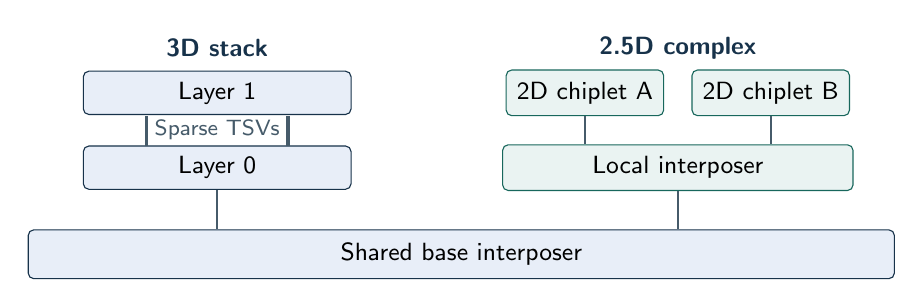
\begin{tikzpicture}[x=1cm,y=1cm,font=\small\sffamily,
  planar/.style={draw=Link,rounded corners=2pt,fill=Panel,minimum width=2cm,minimum height=.58cm},
  layer/.style={draw=Heading,rounded corners=2pt,fill=Stack,minimum width=3.4cm,minimum height=.55cm},
  conn/.style={draw=Muted,line width=.7pt}]
  \node[draw=Heading,rounded corners=2pt,fill=Stack,minimum width=11cm,minimum height=.62cm] (base) at (0,0) {Shared base interposer};
  \node[layer] (l0) at (-3.1,1.1) {Layer 0};
  \node[layer] (l1) at (-3.1,2.05) {Layer 1};
  \draw[conn] (l0.south) -- (-3.1,.32);
  \draw[conn,line width=1.15pt] (-4,1.38) -- (-4,1.76);
  \draw[conn,line width=1.15pt] (-2.2,1.38) -- (-2.2,1.76);
  \node[font=\footnotesize\sffamily,text=Muted] at (-3.1,1.575) {Sparse TSVs};
  \node[font=\small\sffamily\bfseries,text=Heading] at (-3.1,2.62) {3D stack};

  \node[planar,minimum width=4.45cm] (local) at (2.75,1.1) {Local interposer};
  \node[planar] (chipA) at (1.57,2.05) {2D chiplet A};
  \node[planar] (chipB) at (3.93,2.05) {2D chiplet B};
  \draw[conn] (chipA.south) -- (1.57,1.4);
  \draw[conn] (chipB.south) -- (3.93,1.4);
  \draw[conn] (local.south) -- (2.75,.32);
  \node[font=\small\sffamily\bfseries,text=Heading] at (2.75,2.62) {2.5D complex};
\end{tikzpicture}\\[-1mm]
{\small A stack and a group of planar chiplets connected through a shared base.}
\end{center}

\subsection{What the search has to place}

The input is a weighted application graph. Each vertex is a task, and an edge's weight gives the amount of traffic sent from one task to another. We assign each task to a different router slot. Spare slots carry placeholder IDs with no application traffic. The interposer routers forward packets and are outside the task capacity.

With \(R\times C\) slots per plane, \(H\) layers per stack, and \(W\) planar chiplets per 2.5D group, the task capacity is
\[
N_{\mathrm{slots}}=RC\bigl(H\,n_{\mathrm{3D}}+W\,n_{\mathrm{2.5D}}\bigr).
\]
For instance, one four-layer stack and one four-chiplet group, each using \(2\times2\) planes, give \(4(4+4)=32\) slots. We used this mixed configuration for Graph 4.

\clearpage
\subsection{An actual starting particle}

In PSO, a \emph{particle} is one candidate design. It stores where tasks sit, which TSV columns are installed, which TSV each router uses, and where each unit connects to the base. GA calls the same kind of design a chromosome.

Here is a particle from the baseline PSO generator with seed 10 and elevator-first assignment. Graph 2 has 12 tasks. We gave it eight slots in a \(2\times2\times2\) stack and four in one planar chiplet. This is the \code{chromosome} field of the generated JSON, after the initial repair and before the first search move.

{\small
\begin{verbatim}
{
  "chromosome": [
    [
      [9, 0, 6, 7, 10, 1, 3, 5],
      [1, 0, 0, 1],
      [0, 0, 3, 3, 4, 4, 7, 7],
      2
    ],
    [
      [2, 4, 8, 11],
      0
    ]
  ]
}
\end{verbatim}
}

The first block is the stack. Its first list places task 9 at router 0, task 0 at router 1, and so on. The second list puts TSVs at planar positions 0 and 3. These send traffic between routers \(0\leftrightarrow4\) and \(3\leftrightarrow7\) across the two layers. In the third list, the 0 at index 1 tells router 1 to use TSV router 0 when changing layers. The final value, 2, is the stack's bottom-layer attachment router.

The second block places tasks 2, 4, 8, and 11 on the planar chiplet. The 0 after the list selects local interposer router 0 as the attachment. The JSON metadata records a \(5\times5\) shared base and the base-side connection points at \((1,1)\) and \((4,1)\).

We repair each design at initialization and after a move. The repair keeps each task ID in exactly one slot, checks the number and spacing of the TSV columns, and gives every router a valid TSV on its own layer. A router with a TSV selects itself. Attachment indices also stay within the relevant router range.

To generate this particle from \path{Final/}, run the command below. The last three positional values ask for zero search iterations, one particle, and elevator-first assignment.

{\small
\begin{verbatim}
python3 pso_3p5d.py Graph2 2 2 1 2 1 1 0 1 0 --seed 10
\end{verbatim}
}

\clearpage
\section{How we scored and searched designs}

\subsection{Weighted hops}

We want to shorten the paths that carry the most traffic. For each graph edge from \(a\) to \(b\), we multiply its traffic weight \(b_{ab}\) by the modeled number of hops between their assigned routers \(\pi(a)\) and \(\pi(b)\). The sum is the communication cost.
\[
C=\sum_{(a,b)} b_{ab}\,h\bigl(\pi(a),\pi(b)\bigr).
\]
An edge with weight 20 and a four-hop route contributes 80. Saving one hop on that route saves 20 cost units. The same change on an edge with weight 2 saves two units.

The route length includes the detour to a TSV, the vertical crossing, and the onward path from the arrival router. If the tasks lie in different units, it can also include the local and base interposers and their attachments.

\subsection{How evenly the TSVs are used}

A short placement can still funnel traffic through one TSV. For each route we add its traffic weight to every directed vertical link it traverses. We count upwards and downwards separately on each layer interface. We include installed links that carry no traffic, since they show where there is unused capacity.

For one direction \(d\), let \(L_\ell\) be the traffic on link \(\ell\) and \(\overline L_d\) the mean over its \(m_d\) installed links. We use the population variance
\[
V_d=\frac{1}{m_d}\sum_{\ell=1}^{m_d}(L_\ell-\overline L_d)^2.
\]
A direction with no links contributes zero. Loads of \([12,0]\) have a variance of 36. Loads of \([6,6]\) carry the same total traffic and have a variance of zero.

We corrected the route tracing for native stacks as we developed this measure. Inside a stack, the forwarder can check the TSV selection again at each planar hop. When traffic crosses the base, we trace the source descent and start the destination ascent at the destination's actual attachment. This makes the hop cost and TSV loads follow the same path.

\subsection{The score used by PSO}

We take the larger directional variance so that an imbalance in either direction counts. We put cost and variance on a common scale before giving them equal weights.
\[
F=0.5\,\frac{C}{C_{\mathrm{ref}}}
  +0.5\,\frac{\max(V_{\uparrow},V_{\downarrow})}{V_{\mathrm{ref}}}.
\]
Lower \(F\) is better. The cost reference multiplies the graph's total traffic weight by an upper bound on route cost. The variance reference is the square of the total traffic weight. Later, the simulator measures delay, throughput, and energy with packets moving through the network.

\clearpage
\subsection{Genetic algorithm (GA)}

We start GA with a population of designs. At each generation we score them, keep some of the strongest, and choose parents for crossover. Crossover combines parts of the parents' designs. A mutation changes the mapping or TSV placement so the population can explore again when it stalls. We repair the resulting designs before using them. In the batch runs we raised the stagnation threshold for triggering mutation from 20 to 50 iterations.

\subsection{Simulated annealing (SA and ASA)}

SA works on one design at a time. We make a small move, such as swapping two tasks, reversing part of the mapping list, moving an attachment, or flipping a TSV mask bit and repairing the mask. We accept an improvement. A worse move that increases fitness by \(\Delta F\) can still be accepted with probability \(\exp(-\Delta F/T)\), where \(T\) is the temperature. This gives the search a way out of a local minimum. As the temperature goes down, worse moves become less likely to pass.

We also implemented adaptive simulated annealing (ASA). It uses the same moves but adjusts the temperature based on the fraction of proposals it has recently accepted. We set the default target to 40 percent. It can also reheat after an extended stall.

\subsection{Particle swarm optimization (PSO)}

Each particle remembers its own best design. The swarm also keeps the best design any particle has found. At each iteration, a particle tries some of the swaps that would move it toward those two designs. It can keep swaps from its previous move too.

We represent a velocity as an ordered list of swaps because our task slots hold a permutation. For example, to move \([0,1,2,3]\) toward \([2,0,1,3]\), PSO can swap positions \((0,2)\) and then \((1,2)\). Every swap leaves exactly one copy of each task ID in the mapping. In the baseline, the probabilities for keeping a swap from the previous velocity, the personal best, and the global best are 0.10, 0.04, and 0.02, respectively. The update can also swap entries in a TSV mask or copy a best design's attachment.

After a move we repair and score the particle. We update its personal best and the swarm best when the new score is strictly lower. The final baseline stops at the requested iteration limit or after 100 iterations without a new swarm best. We shortened that stopping threshold during the experiments to avoid continuing a run after a long stall.

\clearpage
\section{Running a placement in Noxim 3.5D}

The pipeline takes the same application from optimization through to the Excel report.

\begin{enumerate}
\setlength{\itemsep}{2pt}
\item Read the application's communication matrix as a weighted edge list. Run the optimizer and save its best particle as JSON.
\item Generate the topology YAML from that particle, including the meshes, TSVs, and interposer connections. Translate each communication edge into a source router, destination router, and packet injection probability. We scale injection weights relative to the largest edge weight.
\item Run Noxim with the topology and traffic table. Read delay, throughput, delivered traffic, and energy from the simulator output.
\item Store one run per CSV row. Batch runs share a file for their algorithm, assignment mode, and start time. The Excel exporter puts placement scores and simulator measurements on separate sheets. The results record optimizer CPU time and wall time separately from simulator time.
\end{enumerate}

\subsection{Why we used depth-first routing}

If source and destination are in different units, a packet can first descend to their common interconnect, then ascend into the destination unit. Inside a stack the forwarder uses the selected TSV on the current layer to reach the next one.

We used \code{DEPTH\_FIRST} because it supports these paths in the hierarchy produced by the topology generator. Our standard setup used two virtual channels and buffer-level selection. A packet on the downward channel can move to the upward channel when it starts to ascend. The implementation prohibits a turn back from the upward channel onto a downward link. Holding the routing policy fixed let us compare the two ways of choosing TSVs for the routers.

\subsection{Run the full pipeline}

Run this from the project directory in Bash on Linux or WSL. It places Graph 4 on the mixed network described earlier and simulates the best particle.

{\small
\begin{verbatim}
source bin/env.sh
python3 run_pipeline.py --algorithm PSO --graph 4 \
  --chiprows 2 --chipcols 2 --two5dwidth 4 --threedheight 4 \
  --num2p5d 1 --num3d 1 --population 100 --iterations 500 \
  --seed 10 --sim-seed 10 --mode random
\end{verbatim}
}

The same launcher accepts \code{GA} and \code{SA}. For native meshes, use \path{native_3d_mesh/run_pipeline_mesh.py} with the topology arguments above. Select elevator-first assignment with \code{--mode elevator}. From Windows Python, use the command on one line and add \code{--use-wsl} to launch the Linux simulator.


\clearpage
\section{Choosing a TSV for each router}

The TSV mask says where vertical links exist. The assignment table tells a router which of those links to use. We tested two ways to build that table.

\textbf{Elevator-first} prefers the nearest eligible TSV by Manhattan distance. It looks for candidates below the assignment-count limit when possible and breaks equal-distance ties using the router ID.

\textbf{Random} follows the REDELF directional rule. It chooses from installed TSVs to the south or due east, again preferring candidates below the assignment limit. A pivot gives the router a fallback when that set is empty. We aligned the seeded selection order with the Tabu-search implementation used for comparison. If the assignments would cause a cycle during native forwarding, the affected layer switches to nearest-TSV assignments.

Suppose a router at \((1,0)\) is one hop from both TSVs at \((0,0)\) and \((1,1)\). With both below the limit, elevator-first chooses the lower ID at \((0,0)\). The random policy can choose only the southern candidate at \((1,1)\) under its directional rule. The two installed columns are the same, but the traffic crosses at a different one.

In the 34 matched PSO runs, elevator-first gave lower communication cost on 23 graphs and higher average IP throughput on 20. Random gave lower average delay on 18 graphs. The assignments can lead PSO to different designs. For example, random's cost on Graph 4 was 16,257, compared with 22,507 for elevator-first. On Graph 10, elevator-first led with 536.607, compared with 746.897. We kept both modes because the better choice changed with the graph and the measure.

\section{Moving to a native 3D mesh}

We first represented a stack as several planar mesh components and joined them with explicit vertical links. For example, a \(3\times3\times4\) stack used four \(3\times3\times1\) components. We then implemented a native \(3\times3\times4\) mesh. It has the same 36 slots, with one component ID range and internal TSVs at the installed columns.

We chose the native mesh for the pure 3D runs because AccessNoxim also uses one mesh for a stack. That gave us a direct way to match a task's \((x,y,z)\) position and the vertical link it uses. The simulator can also tell an internal layer crossing from a trip to another chiplet.

In a mixed 3.5D network, the multi-mesh container still joins stacks, planar chiplets, and interposers. Each stack inside it can be one native mesh. We updated the YAML generator to write internal TSV positions and router assignments, including downward selections to reach a stack's bottom attachment.

\clearpage
\section{Preparing the simulators for comparison}

\subsection{Matching router numbers}

For a traffic-table entry, we need to know where each task sends its packets in the simulator. That requires three numbers. The task ID comes from the application graph. The local router ID identifies a slot inside its mesh. The global router ID identifies that slot across the entire network.

In both simulators, the local numbering for a plane of width \(X\) and height \(Y\) is
\[
\mathrm{localID}(x,y,z)=x+yX+zXY.
\]
Coordinates start at zero and \(x\) changes fastest. In an AccessNoxim run with one mesh, the local ID already identifies the router across the whole network. In a multi-component 3.5D run, we add the component's starting offset. For example, \((1,0,1)\) in a \(2\times2\times2\) mesh is local router 5. If the mesh starts at global ID 9, that router is global ID 14.

The generator inverts the particle's placement list to find the slot that holds each task. It then applies offsets in the simulator's component order, including routers used only by the interposers. For a single stack with no base, it can use the stack numbering directly. We also wrote an AccessNoxim exporter so the same placement and TSV selections can be passed into the 3D simulator.

\subsection{Sizing the interposers}

We made the base interposer depend on the units in the design. The layout builder places the unit footprints on a square grid, with a fixed spacing between them, and grows the grid until all footprints fit. It also sizes the local interposer for a group of planar chiplets. The particle records the dimensions and connection points so the optimizer, YAML generator, and traffic generator use the same geometry.

When there is one stack, we omit the base. This keeps extra routers and links out of the pure 3D energy comparison. For a mixed design, we connect each stack's bottom attachment or each 2.5D group's local attachment to the appropriate base router.

\subsection{Getting runs ready in batches}

We extended the generator to handle rectangular planes, check task capacity, and maintain the correct traffic endpoints when slots are unused. We added two-layer and four-layer native-mesh batches, as well as seeded sampling of a subset of graphs. The launchers let us control buffer depth, packet size, and warm-up, and rerun a given graph with the same optimizer and simulator seeds.

\clearpage
\subsection{What the energy comparison showed}

We compared 21 two-layer cases. The top panel shows the percentage change in reported Noxim 3.5D energy when switching the simulator's \emph{routing policy} from depth-first (DF) to elevator-first (EF). The bottom panel compares AccessNoxim with the mean of the two Noxim 3.5D totals for each graph and mesh. These are routing and simulator comparisons. Section 4 compares \emph{assignments} under a common routing policy.

\[
\mathrm{Routing\ change}=100\,\frac{E_{\mathrm{EF}}-E_{\mathrm{DF}}}{E_{\mathrm{DF}}},
\qquad
\mathrm{Energy\ ratio}=\frac{E_{\mathrm{Access}}}{(E_{\mathrm{DF}}+E_{\mathrm{EF}})/2}.
\]

\begin{center}
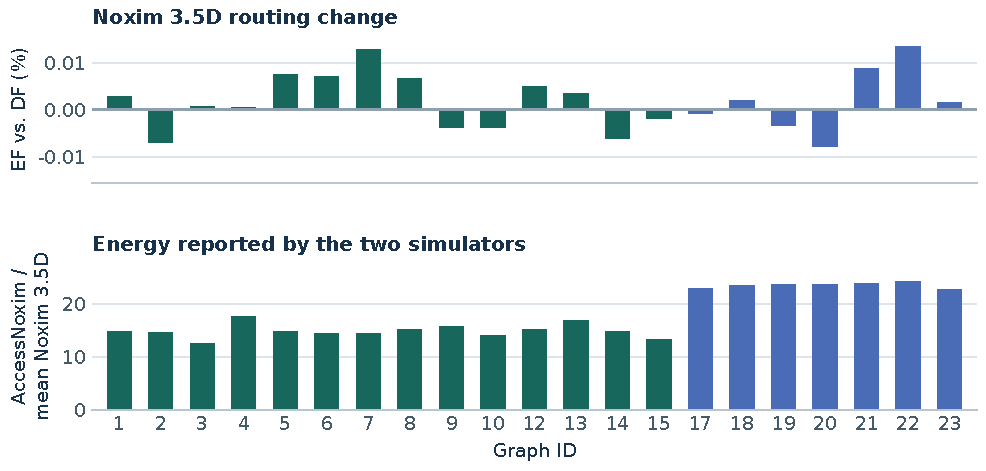
\includegraphics[width=.96\linewidth]{figures/energy-comparison.pdf}\\[-1mm]
{\small Reported energy for the two-layer cases. Graphs 17--23 use \(8\times4\times2\) meshes.}
\end{center}

The two routing policies gave nearly the same total energy. The largest absolute change was \(0.0133\%\), on Graph 22. For these cases, delay, throughput, and delivered traffic are more useful for choosing between the routing policies.

The simulator difference was much larger. AccessNoxim reported between \(12.57\) and \(24.24\) times the mean Noxim 3.5D energy. For Graph 4 on a \(4\times4\times2\) mesh, the totals were \(3{,}760.819\,\mu\mathrm{J}\) in AccessNoxim and \(212.509\,\mu\mathrm{J}\) on average in Noxim 3.5D, a factor of \(17.70\).

We checked how the code accounts for buffers, crossbar transfers, links, virtual channels, and idle leakage. The reported totals establish the size of the gap. To find its cause, the two runs need matched traffic, simulation windows, and power-model settings. Breaking out idle energy and energy per delivered flit would help locate the difference.

\clearpage
\section{Why we carried PSO forward}

We first checked the pipeline through 30 complete runs on Graphs 4 and 62. For the larger comparison, each batch chose a supported mesh size from the task count and ran the same optimization, simulation, and export steps. The main static sheet records a configured population of 1,000 and an iteration limit of 500. It includes 34 graphs under each assignment mode.

We chose PSO mainly on communication cost. Of the three methods, it gave the lowest cost on 29 of 34 graphs in random mode and 32 of 34 in elevator-first mode. GA led the other seven cases, including Graph 10 in random mode. PSO also had the lowest reported normalized TSV variance in 42 of the 68 comparisons.

The Noxim measurements put those scores in context. We matched the benchmark labels for GA, SA, and PSO on 24 graphs in each mode. In random mode, PSO had the highest average IP throughput on 13 and the lowest average delay on 8. In elevator-first mode the counts were 11 and 10. A lower placement cost can help, but packets also queue and compete for links during simulation.

SA had the shortest optimizer CPU time in all 68 static comparisons. That gave us a clear reason to work on PSO's evaluation cost. We kept its search as the baseline so we could see whether caching would speed it up while keeping the resulting designs.

\subsection{Repeat a native mesh batch}

From the project directory in Bash, use the three launchers below. Set \code{MODE} in \path{native_3d_mesh/run_all_mesh_graphs.py} to \code{elevator} or \code{random} before the run. The batch launcher keeps the results together by algorithm, mode, and batch start time.

{\small
\begin{verbatim}
source bin/env.sh
python3 native_3d_mesh/run_ga_mesh_graphs.py
python3 native_3d_mesh/run_sa_mesh_graphs.py
python3 native_3d_mesh/run_pso_mesh_graphs.py
\end{verbatim}
}

\clearpage
\section{Making PSO faster}

An evaluation follows the routes for the application's edges and adds their loads to the TSVs. As PSO progresses, multiple routes can share part of a path and multiple particles can reach the same design. We used these two kinds of repetition to reduce the work.

\subsection{Dynamic programming (DP)}

Consider two routes that reach the same router on layer 1, both headed toward layer 3. If the forwarding condition is the same, the remainder of their vertical traversal is the same. We save that suffix after the first route so the next can reuse it. If \(s\) is the current routing state and \(t\) is the next one, the remaining cost follows
\[
H(s)=c(s,t)+H(t).
\]
At the target layer the remaining vertical traversal costs zero. We then add the final planar distance. The cache key is the current router, the target layer, and whether forwarding keeps the selected TSV until the next crossing. We save the cost, arrival router, and list of directed TSV crossings. That list lets each flow add its own load even when it uses the saved route.

Within one particle, we also cache the distance for an ordered pair of routers. At the swarm level, we cache the score of a complete repaired particle for the given topology, traffic, and normalization. If two repaired designs are identical, we need only one score. The moves, fitness function, and best updates follow the baseline PSO rules.

The workbook's DP results used less optimizer CPU time in all 68 matched cases. The median reduction within graph-and-mode pairs was 38.1\% in random mode and 23.1\% in elevator-first mode. Communication cost matched in 67 cases. The one difference was 0.0005 on a cost of about 1.61 million, on Graph 29 in elevator-first mode.

\subsection{DP with multithreading}

The coordinating thread generates and repairs candidates, looks up scores, and groups repeated candidates. It sends each distinct cache miss to a worker with its own routing context. Once the batch returns, the coordinator records the scores and updates personal and swarm bests in the usual order. Keeping the random choices and best updates ordered makes the seeded search repeatable across worker counts.

Threads are most useful when a batch contains enough independent misses to keep them busy. Serial work, scheduling, and Python's interpreter lock can limit the improvement. We kept serial and threaded DP as separate variants so their elapsed time could be compared with the same inputs, seeds, and worker settings recorded.


\clearpage
\subsection{Trying an extra move with Q-learning}

We tried Q-learning on its own first, using broad states based on the gap to the best design and how long the search had stalled. We also built a prototype combining PSO, DP, and Q-learning. Then we separated the learned move from DP so we could measure what it added to PSO.

In PSO with Q-learning, the state is identified by a hash of the complete repaired particle. An action is a sequence of task or TSV swaps. The learner can also keep the particle as it is. It usually chooses an action with a promising value in the Q-table and occasionally tries a random one.

We first make and score the usual PSO move. Then we choose an action, apply it, repair the result, and score it again. The reward is \(F_{\mathrm{before}}-F_{\mathrm{after}}\). A move from 0.080 to 0.075 earns 0.005. The learner uses that reward and its estimate of the next state's best action to update the value of the move it tried.

This extra pass is where much of the runtime goes. Q-learning scores both the PSO proposal and the design after its edit. It also builds candidate edits, hashes particles, and updates the table. By comparison, DP avoids work when it recognizes a route or design it has already scored. The Q-table holds estimates of which moves might help. In a large search space, some of those estimates will see little reuse because the exact particle may never recur.

\subsection{How much did the learned move help?}

We matched the rows with numeric results for baseline PSO and PSO with Q-learning in the static sheet. Q-learning got a lower communication cost in 20 of 28 random-mode cases and 21 of 26 elevator-first cases. It took more CPU time in 52 of the 54 comparisons. Taking the median of the paired time ratios gives \(2.04\) times baseline PSO in random mode and \(2.37\) times in elevator-first mode.

We saw enough quality gains to keep Q-learning as an experiment. We kept the DP variants as our main implementations because they reduced the work needed to score the same PSO search. An equal-evaluation-budget comparison across several graphs and seeds would help us measure how much of Q-learning's gain comes from its choice of moves when both methods can score the same number of proposals.

\clearpage
\subsection{How much space did the Q-table need?}

For the sweep in \path{results.xlsx}, we ran Graph 4 with seed 10, random TSV assignment, 1,000 particles, 500 iterations, and four evaluation workers. A two-layer stack and two planar chiplets on \(3\times3\) planes gave us 36 slots for 32 tasks. We tried capacities from 0 to 500,000 state rows, increasing by 10,000 each time. At zero the run uses baseline PSO. At a positive capacity, a full table drops the least recently used state to make space.

\begin{center}
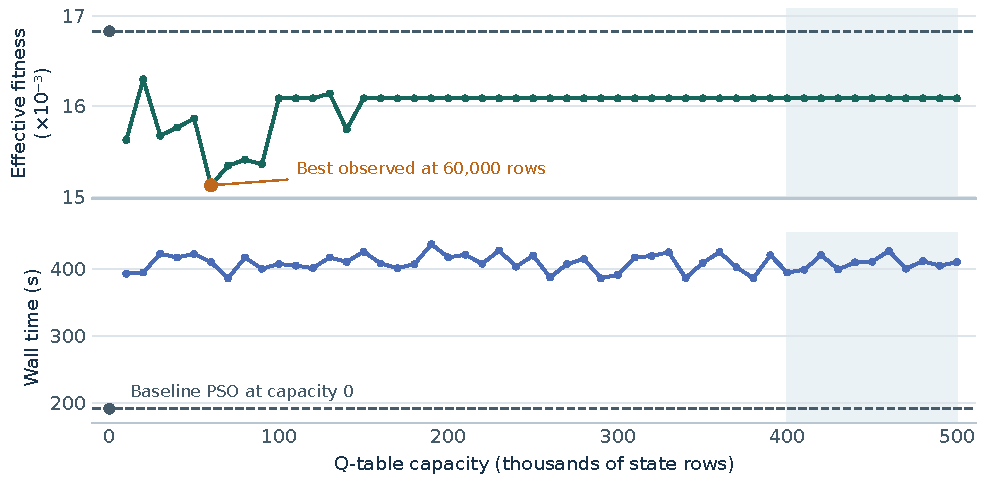
\includegraphics[width=.96\linewidth]{figures/q-table-capacity.pdf}\\[-1mm]
{\small Graph 4 with one run per capacity. The shaded range had zero evictions.}
\end{center}

The lowest fitness was at 60,000 rows. It fell from 0.016829 for baseline PSO to 0.015127, an improvement of 10.1\%. Communication cost fell from 16,257 to 14,845, about 8.7\%. The run took 410.0 seconds, compared with 191.1 seconds for baseline PSO. The fastest Q-learning run was at 70,000 rows. It took 386.0 seconds and reached a fitness of 0.015344.

At 400,000 rows, evictions stopped. Peak occupancy was 397,868 rows, and the best fitness stayed at 0.016087 through 500,000 rows. In this sweep, keeping every state used more table space and still gave a higher fitness than the 60,000-row table.

Every positive capacity beat baseline PSO on fitness for this graph and seed. The base run completed 501,000 fitness evaluations and every Q-learning run completed 1,001,000. Since the sweep held iterations fixed, the two-pass variant had more chances to find an improvement. We would start a repeat study with 60,000 and 70,000 rows because one gave the best score and the other the shortest Q-learning run in this sweep.

\clearpage
\section{The three versions we kept}

\begin{itemize}
\setlength{\itemsep}{3pt}
\item \textbf{Baseline PSO (\code{PSO}).} This is the reference search. It scores the repaired particles serially.
\item \textbf{PSO with DP (\code{PSO\_DP}).} This version reuses route segments and scores for identical designs. It evaluates the remaining candidates serially.
\item \textbf{PSO with DP and multithreading (\code{PSO\_DP\_MT}).} This version adds workers to score the distinct candidates that miss the cache.
\end{itemize}

We put all three in \path{Final/} with the topology, traffic, and export scripts. They use the benchmark graphs and simulator from the parent project. To try every variant on a small native 3D mesh, run this from the project directory in Bash.

{\small
\begin{verbatim}
cd Final
python3 run_pipeline.py --algorithm ALL --graph 3 \
  --chiprows 2 --chipcols 2 --two5dwidth 1 --threedheight 2 \
  --num2p5d 0 --num3d 1 --population 8 --iterations 12 \
  --seed 10 --sim-seed 11 --parallel-workers 4 --native-3d-mesh
\end{verbatim}
}

The command produces a CSV and Excel workbook for each variant and one Excel workbook comparing all three. To run just one version, replace \code{ALL} with its name. The \path{Final/README.md} describes the output locations and how to repeat just the simulation or Excel export. The theory guide in \path{Final/PSO.pdf} gives the detailed update and evaluation rules.

We checked the packaged pipeline on Graphs 3 and 4. The project tests cover TSV validity, directional variance, cache reuse, consistent results across worker counts, and Q-table capacity.

\section{Results and code}

The benchmark workbook contains the full placement and simulation measurements. \href{https://docs.google.com/spreadsheets/d/13I29-_UOsBwOk56806ZpmFxmFg6YCexZC1dRvwPh1W8/edit?gid=0#gid=0}{Open the benchmark workbook}.

The Q-table sweep is in \path{results.xlsx}. It includes the run settings, wall times, fitness, communication cost, occupancy, evictions, and evaluation counts.

The repository contains the simulator integration and the implementations discussed in this report. \href{https://github.com/RagavKrishnaRamesh/3.5D-NOC-Simulator-Code}{Open the project on GitHub}.

\end{document}
